\documentclass[a2paper,landscape,fontscale=0.545]{baposter}

\usepackage{microtype}
\usepackage{palatino}
\usepackage{graphicx}
\usepackage{multicol}
\usepackage{amsmath}
\usepackage{amssymb}
\usepackage{mathtools}
\usepackage{wrapfig}
%\usepackage{hyperref}

\begin{document}

%\definecolor{lightpurple}{rgb}{0.145,0.6666,1}
\definecolor{purple}{RGB}{126,49,123}
\begin{poster}%
  % Poster Options
  {
  % Show grid to help with alignment
  grid=false,
  columns=3,
  % Column spacing
  colspacing=0.8em,
  % Color style
  bgColorOne=white,
  bgColorTwo=white,
  borderColor=purple,
  headerColorOne=black,
  headerColorTwo=purple,
  headerFontColor=white,
  boxColorOne=white,
  boxColorTwo=purple,
  % Format of textbox
  textborder=roundedleft,
  % Format of text header
  eyecatcher=true,
  headerborder=closed,
  headerheight=0.1\textheight,
%  textfont=\sc, An example of changing the text font
  headershape=roundedright,
  headershade=shadelr,
  headerfont=\textsc, %Sans Serif
  textfont={\setlength{\parindent}{1.5em}},
  boxshade=plain,
%  background=shade-tb,
  background=plain,
  linewidth=2pt
  }
  % Eye Catcher
  {eyecatcher=no} 
  % Title
  {Relativity and the Global Positioning System}
  % Authors
  {James Fielder \\ Supervised by Prof. Richard Ward}
  % University logo
  {
    \includegraphics[height=4.0em]{images/dur_logo.pdf}
  }


\headerbox{Fundamentals of GPS}{name=fundamentals,column=0,row=0}{
\noindent GPS fundamentally relies on the consistency of the speed of light in any inertial frame. Given the positions $\vec{r}_i$ and times $t_i$ of four GPS satellites a receiver can determine their position $\vec{r}$ and time $t$ using:
\vspace{-0.7em}
\[ c^2 (t-t_i)^2 = |\vec{r}-\vec{r}_i|^2 \]
\noindent While the relativistic effects on the system are fairly small, the clock on the satellites only need to be out by $3\text{ns}$ for there to be an error of 1m to the calculation of position. 
}

\headerbox{Relativistic Errors}{name=errors,column=0,below=fundamentals}{
\noindent There are 4 main sources of relativistic errors in the GPS:
\vspace{-0.5em}
\begin{itemize}
  \item Time dilation due to the motion of the satellites \vspace{-0.5em}
  \item Gravitational time dilation \vspace{-0.5em}
  \item The Sagnac effect \vspace{-0.5em}
  \item Doppler shifts in radio frequencies \vspace{-0.3em}
\end{itemize}  
}

\headerbox{Time Dilation due to Satellite Motion}{name=SR,column=0,below=errors}{
\noindent If we consider a stationary observer on (but not moving with) the earth measuring the velocity of a GPS satellite they find that the velocity of a satellite $v_s$ is approximately $3900$m/s. Thus by using the special relativistic time dilation formula $\gamma_s = \left(1 - \frac{v_s^2}{c^2}\right)^{-1/2}$ we find that the fractional change in time compared to a motionless clock is $0.85 \times 10^{-10}$. Here we can safely ignore the motion of a clock due to the rate of the earth, as it has a corresponding value of $\gamma$ which is over 100 times smaller than for the satellites.
}

\headerbox{Sagnac Effect}{name=sagnac,column=1,span=2}{
\noindent The sagnac effect is caused by the motion of the earth. As an observer on the surface of the earth receives signals from the satellites in orbit we must correct for if the satellite is ahead of the motion of the earth or behind it. Consider the standard Minkowski line element $-ds^2 = -(c dt)^2 + dr^2 + r^2 d\phi^2 + dz^2$ in cylindrical coordinates. Transform this to an equivalent flat space but with the azimuthal coordinate rotating with angular speed $\omega_{e}$: 
\vspace{-0.9em}
  \[-ds^2 = - \left(1- \frac{\omega_{e}^2 {r'}^2}{c^2}\right)(cdt')^2 + 2 \omega_{e} {r'}^2 d\phi' dt' + (d\sigma')^2\]

\noindent with $(d\sigma')^2 = (dr')^2 + (r' d \phi')^2 + (dz')^2$. Light travels such that $ds^2 = 0$. If we ignore terms $\frac{\omega_{e}^2 {r'}^2}{c^2} << 1$ we can solve for $dt'$ and integrate to obtain the time of travel: 
\[\int_{path} dt' = \int_{path} \frac{d \sigma'}{c} + \frac{2\omega_{e}}{c^2} \int_{path} d {A'}_{z} \]
\noindent where $dA_z$ is the projection of the path taken by an observer on the surface of the earth projected onto a triangular infinitesimal area on a plane through the equator. Thus we observe that the Sagnac effect is dependent on how close you are to the equator: for observers at the pole no such effect would be measured, whereas for observers at the equator this could amount to a discrepancy in measured time from the satellite of up to $\pm 207 $ns. 
}

\headerbox{Sagnac Effect Diagram}{name=sagnac-dia,column=2,below=sagnac}{
\begin{center}
%\begin{figure}
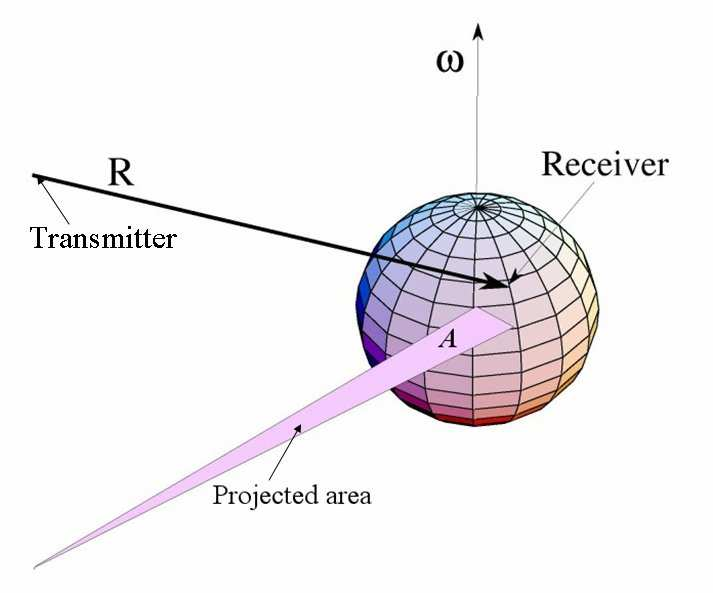
\includegraphics[scale=0.25]{images/sagnac.png}
%\caption{Projection of $A_z$ taken from Ashby's article}
%\end{figure}

Diagram of the projection onto $A_z$ taken from Ashby's article.
\end{center}
}

\headerbox{Gravitational Time Dilation}{name=GR-T,column=1,below=sagnac,aligned=SR}{
\noindent Gravitational time dilation states that a clock in a higher gravitational potential will run faster than a clock in a lower potential. As such there will be an effect contrary to the special relativistic effect slowing the satellite clocks down, due to the satellites being at a higher potential than the surface of the earth. This effect is given by \[ \frac{\Phi_{E} - \Phi_{s}}{c^2}\] with $\Phi_{E}$ the potential at the earth's surface and $\Phi_{s}$ the potential at the satellite. By taking $\Phi = - \frac{GM}{r}$ (the standard Newtonian potential) we find that this effect corresponds to a fractional change in time of $-5.2 \times 10^{-10}$. This is far larger than the special relativistic result. Thus we see that the GPS depends not only on special relativistic physics but also on general relativity.  
}

\headerbox{References}{name=ref,column=1,below=GR-T}{
{\footnotesize
\noindent Relativity, Gravitation and Cosmology - Ta-Pei Cheng

\noindent Gravity: An introduction to Einstein's Relativity - James B. Hartle

\noindent Relativity in the Global Positioning System - Neil Ashby - \\ http://www.livingreviews.org/lrr-2003-1

\noindent Global Positioning System: Theory and Applications Vol 1 - Neil Ashby and James Spilker - pages 623 - 697
}
}

\headerbox{Doppler Effect}{name=doppler,column=0,below=SR}{
\noindent Due to the high speed of the orbiting satellites relativistic Doppler effects have to be considered when detecting signals from the satellites. The relativistic frequency shift is given by \[f = f_0 \frac{\sqrt{1-v_s^2}}{1 - v_s \cos \alpha}\] where $v_s$ is the velocity of the satellite, $\alpha$ is the angle of the light ray from the satellite's motion. For the main L$_1$ = 1575.42MHz carrier frequency which is used for most of the sending of GPS data this gives potential offsets of up to $\pm 10$KHz which the receivers must account for.
}

\headerbox{Conclusions}{name=conc,column=2,below=sagnac-dia}{
\noindent The Global Positioning System would not be able to function without careful analysis of the physics using relativistic concepts. This poster has only touched on the main issues which relativity brings up: an interested reader is directed to the article by Ashby which describes in depth several other effects which make themselves known in the Global Positioning System.
}

\end{poster}
\end{document}
